\begin{exercises} 

\item Consider the solid $S$ that is bounded by the parabolic cylinder $y = x^2$ and the planes $z=0$ and $z=1-y$ as shown in Figure \ref{F:11.7.TI_Example_2}. 
\begin{figure}[ht]
\begin{center}
%\resizebox{!}{2.0in}{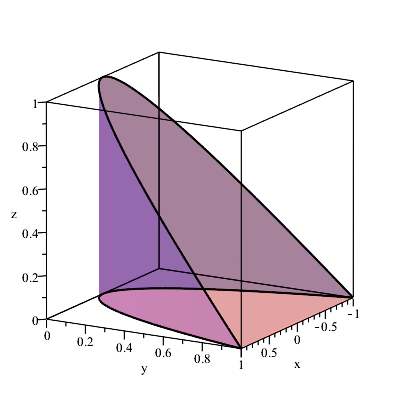
\includegraphics{11_7_TI_Example_2}}
  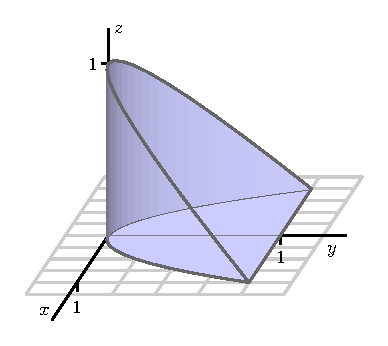
\includegraphics{figures/fig_11_7_solid.eps}
\end{center}
\caption{The solid bounded by $y = x^2$ and the planes $z=0$ and $z=1-y$.}
\label{F:11.7.TI_Example_2}
\end{figure}

Assume the density of $S$ is given by $\delta(x,y,z) = z$
    \ba
    \item Set up (but do not evaluate) an iterated integral that represents the mass of $S$.  Integrate first with respect to $z$, then $y$, then $x$.  A picture of the projection of $S$ onto the $xy$-plane is shown in Figure \ref{F:11.7.TI_Example_2_xy}.

    \item Set up (but do not evaluate) an iterated integral that represents the mass of $S$.  In this case, integrate first with respect to $y$, then $z$, then $x$.  A picture of the projection of $S$ onto the $xz$-plane is shown in Figure \ref{F:11.7.TI_Example_2_xz}.

	\item Set up (but do not evaluate) an iterated integral that represents the mass of $S$.  For this integral, integrate first with respect to $x$, then $y$, then $z$.  A picture of the projection of $S$ onto the $yz$-plane is shown in Figure \ref{F:11.7.TI_Example_2_xz}.

	\item Which of these three orders of integration is the most natural to you?  Why?

	\ea

\begin{figure}[ht]
\begin{center}
\begin{minipage}{1.75in}
\begin{center}
%\resizebox{!}{1.7in}{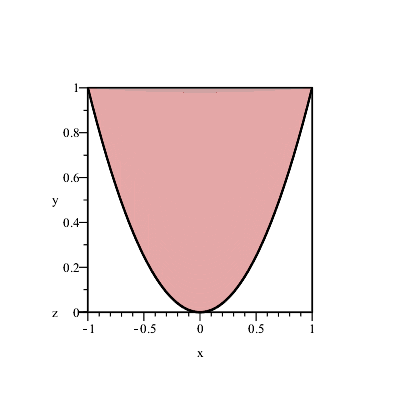
\includegraphics{11_7_TI_Example_2_xy}}
  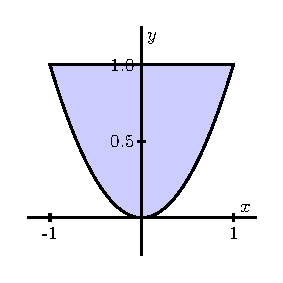
\includegraphics{figures/fig_11_7_solid_proj_1.eps}
\end{center}
\caption{Projecting $S$ onto the $xy$-plane.}
\label{F:11.7.TI_Example_2_xy}
\end{minipage} \hspace{0.1in}
\begin{minipage}{1.75in}
\begin{center}
%\resizebox{!}{1.7in}{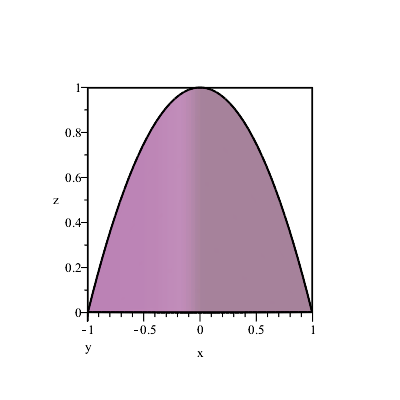
\includegraphics{11_7_TI_Example_2_xz}}
  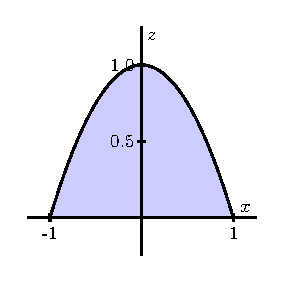
\includegraphics{figures/fig_11_7_solid_proj_2.eps}
\end{center}
\caption{Projecting $S$ onto the $xz$-plane.}
\label{F:11.7.TI_Example_2_xz}
\end{minipage} \hspace{0.1in}
\begin{minipage}{1.75in}
\begin{center}
%\resizebox{!}{1.7in}{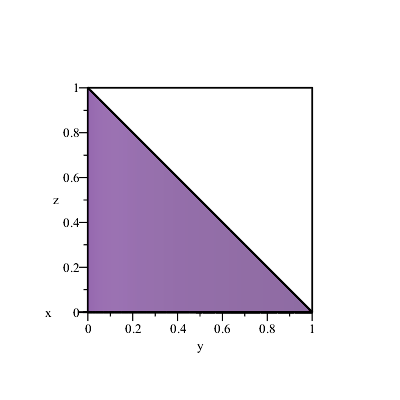
\includegraphics{11_7_TI_Example_2_yz}}
  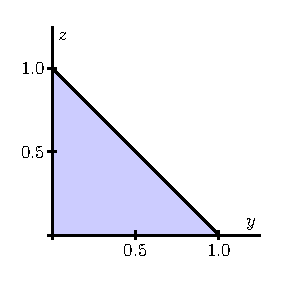
\includegraphics{figures/fig_11_7_solid_proj_3.eps}
\end{center}
\caption{Projecting $S$ onto the $yz$-plane.}
\label{F:11.7.TI_Example_2_yz}
\end{minipage}
\end{center}
\end{figure}

\begin{exerciseSolution}
    \ba
    \item The iterated integral is 
\[\int_{-1}^{1} \int_{x^2}^{1} \int_{0}^{1-y} z \, dz \, dy \, dx.\]

    \item The iterated integral is 
\[\int_{-1}^{1} \int_{0}^{1-x^2} \int_{x^2}^{1-z} z \, dy \, dz \, dx.\]

	\item The iterated integral is 
\[\int_{0}^{1} \int_{0}^{1-z} \int_{-\sqrt{y}}^{\sqrt{y}} z \, dx \, dy \, dz.\]

	\ea
\end{exerciseSolution}

\item This problem asks you to investigate the average value of some different quantities.

	\ba
		\item Set up, but do not evaluate, an iterated integral expression whose value is the average sum of all real numbers $x$, $y$, and $z$ that have the following property: $y$ is between 0 and 2, $x$ is greater than or equal to 0 but cannot exceed $2y$, and $z$ is greater than or equal to 0 but cannot exceed $x+y$.
		\item Set up, but do not evaluate, an integral expression whose value represents the average value of the function $f(x,y,z) = x + y + z$ over the solid region in the first octant bounded by the surface $z = 4 - x - y^2$ and the coordinate planes $x=0$, $y=0$, $z=0$. 
		\item How are the quantities in (a) and (b) similar?  How are they different?
	\ea
	
\begin{exerciseSolution}
\ba
\item We want the average value of the sum $x+y+z$ over the region described. This average value is given by 
\[\frac{\int_0^2 \int_0^{2y} \int_0^{x+y} x+y+z \, dz \, dx \, dy}{\int_0^2 \int_0^{2y} \int_0^{x+y} 1 \, dz \, dx \, dy}.\]
\item We will integrate $x+y+z$ for $z$ from $0$ to $4-x-y^2$. To find the limits on $x$ and $y$, we project $z$ into the $x$-$y$ plane to the parabola $0 = 4 - x- y^2$ or $x = 4-y^2$. Since we are restricted to the first octant, the average value of $f(x,y,z)$ over this region is 
\[\frac{\int_0^2 \int_0^{4-y^2} \int_0^{4-x-y^2} x+y+z \, dz \, dx \, dy}{\int_0^2 \int_0^{4-y^2} \int_0^{4-x-y^2} 1 \, dz \, dx \, dy}.\]
\ea
\end{exerciseSolution}

\item Consider the solid that lies between the paraboloids $z = g(x,y) = x^2 + y^2$ and $z = f(x,y) = 8 - 3x^2 - 3y^2$.

	\ba
		\item By eliminating the variable $z$, determine the curve of intersection between the two paraboloids, and sketch this curve in the $x$-$y$ plane.
		\item Set up, but do not evaluate, an iterated integral expression whose value determine the mass of the solid, integrating first with respect to $x$, then $y$, then $z$. Assume the the solid's density is given by $\delta(x,y,z) = \frac{1}{x^2 + y^2 + z^2 + 1}$.
		\item Set up, but do not evaluate, iterated integral expressions whose values determine the mass of the solid using all possible remaining orders of integration. Use $\delta(x,y,z) = \frac{1}{x^2 + y^2 + z^2 + 1}$ as the density of the solid.
		\item Set up, but do not evaluate, iterated integral expressions whose values determine the center of mass of the solid. Again, assume the the solid's density is given by $\delta(x,y,z) = \frac{1}{x^2 + y^2 + z^2 + 1}$.
		\item Which coordinates of the center of mass can you determine \emph{without} evaluating any integral expression?  Why?
	\ea

\begin{exerciseSolution}
	\ba
		\item Setting $g(x,y)$ equal to $f(x,y)$ we see that the curve of intersection between the two paraboloids is given by $x^2+y^2 = 8-3x^2-3y^2$ or $x^2+y^2=2$. This is the circle centered at the origin with radius $\sqrt{2}$. 
		\item To find mass, we integrate density. An iterated integral whose value represent the mass of the solid is
\[\int_{-\sqrt{2}}^{\sqrt{2}} \int_{-\sqrt{2-x^2}}^{\sqrt{2-x^2}} \int_{x^2+y^2}^{8-3x^2-3y^2} \frac{1}{x^2 + y^2 + z^2 + 1} \, dz \, dy \, dx.\]
		\item If we interchange the orders of $y$ and $x$, then symmetry shows that the mass of the solid is given by 
\[\int_{-\sqrt{2}}^{\sqrt{2}} \int_{-\sqrt{2-y^2}}^{\sqrt{2-y^2}} \int_{x^2+y^2}^{8-3x^2-3y^2} \frac{1}{x^2 + y^2 + z^2 + 1} \, dz \, dx \, dy.\]
To integrate with respect to $y$ first, notice that the limits on $y$ will vary depending on the height. If $0 \leq z \leq 2$, then the limits on $y$ are determined by the paraboloid $z = x^2+y^2$. In this case we have $-\sqrt{z-x^2} \leq y \leq \sqrt{z-x^2}$. When we project this part of the surface onto the $x$-$z$ plane, the result is the parabola $z=x^2$. We want the region above this parabola and below $z=2$. If $2 \leq z \leq 8$, then the limits on $y$ are determined by the paraboloid $z = 8-3x^2-3y^2$. In this case we have $-\sqrt{8-z-3x^2} \leq y \leq \sqrt{8-z-3x^2}$. When we project this part of the surface onto the $x$-$z$ plane, the result is the parabola $z=8-3x^2$. We want the region below this parabola and above $z=2$. So the mass of the solid is given by 
\[\int_{-\sqrt{2}}^{\sqrt{2}} \int_{x^2}^{2} \int_{-\sqrt{z-x^2}}^{\sqrt{z-x^2}} \frac{1}{x^2 + y^2 + z^2 + 1} \, dy \, dz \, dx + \int_{-\sqrt{2}}^{\sqrt{2}} \int_{2}^{8-3x^2} \int_{-\sqrt{\frac{1}{3}(8-z-3x^2)}}^{\sqrt{\frac{1}{3}(8-z-3x^2)}} \frac{1}{x^2 + y^2 + z^2 + 1} \, dy \, dz \, dx .\]


Interchanging the orders of $x$ and $z$ shows that the mass of the solid is given by 
\[\int_{0}^{2} \int_{-\sqrt{z}}^{\sqrt{z}} \int_{-\sqrt{z-x^2}}^{\sqrt{z-x^2}} \frac{1}{x^2 + y^2 + z^2 + 1} \, dy \, dx \, dz + \int_{2}^{8} \int_{-\sqrt{\frac{1}{3}(8-z)}}^{\sqrt{\frac{1}{3}(8-z)}} \int_{-\sqrt{\frac{1}{3}(8-z-3x^2)}}^{\sqrt{\frac{1}{3}(8-z-3x^2)}} \frac{1}{x^2 + y^2 + z^2 + 1} \, dy \, dx \, dz .\]

Finally, we integrate with respect to $x$ first. The symmetry in the surface indicates that these integrals will be similar to ones with $y$ first. So the mass of the solid is also given by 
\[\int_{-\sqrt{2}}^{\sqrt{2}} \int_{y^2}^{2} \int_{-\sqrt{z-y^2}}^{\sqrt{z-y^2}} \frac{1}{x^2 + y^2 + z^2 + 1} \, dx \, dz \, dy + \int_{-\sqrt{2}}^{\sqrt{2}} \int_{2}^{8-3y^2} \int_{-\sqrt{\frac{1}{3}(8-z-3y^2)}}^{\sqrt{\frac{1}{3}(8-z-3y^2)}} \frac{1}{x^2 + y^2 + z^2 + 1} \, dx \, dz \, dy\]
and
\[\int_{0}^{2} \int_{-\sqrt{z}}^{\sqrt{z}} \int_{-\sqrt{z-y^2}}^{\sqrt{z-y^2}} \frac{1}{x^2 + y^2 + z^2 + 1} \, dx \, dy \, dz + \int_{2}^{8} \int_{-\sqrt{\frac{1}{3}(8-z)}}^{\sqrt{\frac{1}{3}(8-z)}} \int_{-\sqrt{\frac{1}{3}(8-z-3y^2)}}^{\sqrt{\frac{1}{3}(8-z-3y^2)}} \frac{1}{x^2 + y^2 + z^2 + 1} \, dx \, dy \, dz .\]

		\item If $M$ is the mass of the solid from part (b), then the center of mass $(\overline{x}, \overline{y}, \overline{z})$ is given by
\begin{align*}
\overline{x} &= \frac{1}{M} \int_{-\sqrt{2}}^{\sqrt{2}} \int_{-\sqrt{2-x^2}}^{\sqrt{2-x^2}} \int_{x^2+y^2}^{8-3x^2-3y^2} \frac{x}{x^2 + y^2 + z^2 + 1} \, dz \, dy \, dx  \\
\overline{y} &= \frac{1}{M} \int_{-\sqrt{2}}^{\sqrt{2}} \int_{-\sqrt{2-x^2}}^{\sqrt{2-x^2}} \int_{x^2+y^2}^{8-3x^2-3y^2} \frac{y}{x^2 + y^2 + z^2 + 1} \, dz \, dy \, dx \\
\overline{z} &= \frac{1}{M} \int_{-\sqrt{2}}^{\sqrt{2}} \int_{-\sqrt{2-x^2}}^{\sqrt{2-x^2}} \int_{x^2+y^2}^{8-3x^2-3y^2} \frac{z}{x^2 + y^2 + z^2 + 1} \, dz \, dy \, dx.
\end{align*}

		\item There is symmetry around the $z$-axis, so we should expect $\overline{z} = 0$. 
	\ea
\end{exerciseSolution}

\item In each of the following problems, your task is to 
	\begin{itemize}
	\item[(i)] sketch, by hand, the region over which you integrate
	\item[(ii)] set up iterated integral expressions which, when evaluated, will determine the value sought  
	\item[(iii)] use appropriate technology to evaluate each iterated integral expression you develop
	\end{itemize}
Note well:  in some problems you may be able to use a double rather than a triple integral, and polar coordinates may be helpful in some cases.	
\ba

	\item Consider the solid created by the region enclosed by the circular paraboloid $z = 4 - x^2 - y^2$ over the region $R$ in the $x$-$y$ plane enclosed by $y = -x$ and the circle $x^2 + y^2 = 4$ in the first, second, and fourth quadrants. 
	
	Determine the solid's volume.

    \item Consider the solid region that lies beneath the circular paraboloid $z = 9 - x^2 - y^2$ over the triangular region between $y = x$, $y = 2x$, and $y = 1$.   Assuming that the solid has its density at point $(x,y,z)$ given by $\delta(x,y,z) = xyz + 1$, measured in grams per cubic cm, determine the center of mass of the solid.

	\item In a certain room in a house, the walls can be thought of as being formed by the lines $y = 0$, $y = 12 + x/4$, $x = 0$, and $x = 12$, where length is measured in feet.  In addition, the ceiling of the room is vaulted and is determined by the plane $z = 16 - x/6 - y/3$.  A heater is stationed in the corner of the room at $(0,0,0)$ and causes the temperature in the room at a particular time to be given by the function
$$T(x,y,z) = \frac{80}{1 + \frac{x^2}{1000} + \frac{y^2}{1000} + \frac{z^2}{1000}}$$	
What is the average temperature in the room?


	\item Consider the solid enclosed by the cylinder $x^2 + y^2 = 9$ and the planes $y + z = 5$ and $z = 1$.   Assuming that the solid's density is given by $\delta(x,y,z) = \sqrt{x^2 + y^2}$, find the mass and center of mass of the solid.

\ea

\begin{exerciseSolution}
\ba

	\item We use polar coordinates with $f(r,\theta) = 4-r^2$ and evaluate with a computer algebra system to see that the volume of the solid is 
\[\int_{-\pi/4}^{\pi/4} \int_0^2 r(4-r^2) \, dr \, d\theta = 2\pi.\]

    \item Using a computer algebra system we find that the mass of the solid is
\[M=\int_0^1 \int_{y/2}^{y} \int_0^{9-x^2-y^2} xyz+1 \, dz \, dx \, dy = \frac{30707}{6144}.\]
The center of mass is then $(\overline{x}, \overline{y}, \overline{z})$ where 
\begin{align*}
\overline{x} &= \frac{1}{M} \int_0^1 \int_{y/2}^{y} \int_0^{9-x^2-y^2} x(xyz+1) \, dz \, dx \, dy = \frac{785256}{1074745} \approx 0.56 \\
\overline{y} &= \frac{1}{M} \int_0^1 \int_{y/2}^{y} \int_0^{9-x^2-y^2} y(xyz+1) \, dz \, dx \, dy = \frac{770584}{1381815} \approx 0.73 \\
\overline{z} &= \frac{1}{M} \int_0^1 \int_{y/2}^{y} \int_0^{9-x^2-y^2} z(xyz+1) \, dz \, dx \, dy = \frac{4438823}{921210} \approx 4.82.
\end{align*}


	\item The volume of the room is 
\[V=\int_0^{12} \int_0^{12-x/4} 16-x/6-y/3 \, dy  \, dx = 1674,\]
so the average temperature in the room is 
\[\frac{1}{V} \int_0^{12} \int_0^{12-x/4} \int_0^{16-x/6-y/3} \frac{80}{1 + \frac{x^2}{1000} + \frac{y^2}{1000} + \frac{z^2}{1000}} \, dz \, dy \, dx \approx 70.52.\]


	\item Since $y$ lies between $-3$ and $3$ on the cylinder, it follows that the plane $z = 5-y$ lies above the plane $z=1$. The mass of the solid is found using cylindrical coordinates as 
\[M = \int_0^{2\pi} \int_0^3 \int_1^{5-r\sin(\theta)} r^2 \, dz \, dr \, d\theta = 72 \pi.\]
The center of mass is then $(\overline{x}, \overline{y}, \overline{z})$ where 
\begin{align*}
\overline{x} &= \frac{1}{M} \int_0^{2\pi} \int_0^3 \int_1^{5-r\sin(\theta)} r^3\cos(\theta) \, dz \, dr \, d\theta = 0 \\
\overline{y} &= \frac{1}{M} \int_0^{2\pi} \int_0^3 \int_1^{5-r\sin(\theta)} r^3\sin(\theta) \, dz \, dr \, d\theta = -\frac{27}{40} \\
\overline{z} &= \frac{1}{M} \int_0^{2\pi} \int_0^3 \int_1^{5-r\sin(\theta)} r^2z \, dz \, dr \, d\theta = \frac{267}{80}.
\end{align*}


\ea
\end{exerciseSolution}

\end{exercises}
\afterexercises
